\documentclass[11pt,a4paper]{article}

% Packages
\usepackage[utf8]{inputenc}
\usepackage[T1]{fontenc}
\usepackage{amsmath,amssymb,amsfonts}
\usepackage{graphicx}
\usepackage{booktabs}
\usepackage{hyperref}
\usepackage{xcolor}
\usepackage{listings}
\usepackage{algorithm}
\usepackage{algpseudocode}
\usepackage{tikz}
\usepackage{geometry}
\usepackage{natbib}
\usepackage{caption}
\usepackage{subcaption}
\usepackage{float}

\geometry{margin=1in}

% Code listing style
\lstset{
    basicstyle=\ttfamily\small,
    keywordstyle=\color{blue},
    commentstyle=\color{gray},
    stringstyle=\color{red},
    showstringspaces=false,
    breaklines=true,
    frame=single,
    numbers=left,
    numberstyle=\tiny\color{gray},
    language=Python
}

% Custom commands
\newcommand{\swifttd}{\textsc{SwiftTD}}
\newcommand{\neuroswift}{\textsc{NeuroSwift}}

\title{Real-Time Neuro-Symbolic Grounding via Asynchronous VLM Supervision\\
\large \neuroswift{}: Bridging Semantic Understanding and Real-Time Control}

\author{Brad Lishman\\
Algodyne Labs\\
\texttt{brad.lishman@algodyne.com}}

\date{}

\begin{document}

\maketitle

\begin{abstract}
Vision-Language Models (VLMs) can provide semantic priors for reinforcement learning, but their latency ($\sim$2s/query) makes frame-by-frame integration impractical for real-time control. We propose a dual-process architecture combining fast temporal-difference learning ({$>$}1000Hz on CPU) with sparse VLM queries triggered only when novel visual features are recruited. The VLM initializes feature weights based on semantic valence (e.g., ``fire'' $\rightarrow$ negative), which the RL agent then refines through experience.

We evaluate on grid navigation with dangerous tiles. Our Imprint-Trigger mechanism achieves \textbf{9--107$\times$ query reduction} compared to frame-by-frame querying while maintaining equivalent task performance (Welch's t-test, $p > 0.3$, non-significant). VLM-initialized agents show \textbf{0\% first-episode deaths} versus 40\% for uninformed agents when encountering fire (Fisher's exact test, $p = 0.001$). Importantly, incorrect VLM priors (``hallucinations'') produce no measurable performance degradation, demonstrating that soft semantic initialization is robust to VLM errors.
\end{abstract}

\section{Introduction}

\subsection{The Semantic Blindness Problem}

Reinforcement learning agents operating in visual environments face a fundamental challenge: they must learn the meaning of visual features through trial and error. A human instantly recognizes fire as dangerous, but an RL agent must step into flames---potentially many times---before learning to avoid them.

This ``semantic blindness'' is costly:
\begin{itemize}
    \item \textbf{Sample inefficiency}: Learning danger through experience requires experiencing danger
    \item \textbf{Safety violations}: First encounters with hazards result in failures
    \item \textbf{Slow adaptation}: Novel objects require extensive interaction before proper valuation
\end{itemize}

\subsection{The VLM Latency Problem}

Vision-Language Models (VLMs) like LLaVA, GPT-4V, and Moondream can provide instant semantic understanding. They know that fire is dangerous, water is often safe, and green goals are desirable. However, VLM inference is slow:

\begin{table}[h]
\centering
\caption{VLM Latency and Cost Comparison}
\begin{tabular}{lcc}
\toprule
\textbf{Model} & \textbf{Latency} & \textbf{Cost} \\
\midrule
GPT-4V & $\sim$3--5s & \$0.01/query \\
LLaVA-7B (local) & $\sim$2s & Compute \\
Moondream (local) & $\sim$1s & Compute \\
\bottomrule
\end{tabular}
\label{tab:vlm_latency}
\end{table}

Real-time control requires decisions at 60Hz (16ms) or faster. Waiting 2 seconds for a VLM response is not viable for reactive behavior.

\subsection{Our Contribution: Asynchronous Semantic Grounding}

We propose a dual-process architecture that separates:

\begin{enumerate}
    \item \textbf{System 1 (Fast)}: \swifttd{} agent running at {$>$}1000Hz, making real-time decisions using tile-coded features with adaptive learning rates
    \item \textbf{System 2 (Slow)}: Frozen VLM queried asynchronously only when novel visual features are detected
\end{enumerate}

The key insight is the \textbf{Imprint-Trigger mechanism}: query the VLM only when the agent encounters a genuinely new visual feature, then use the VLM's semantic assessment to initialize the corresponding weight. Direct experience naturally corrects any VLM errors through TD learning.

\paragraph{Contributions:}
\begin{enumerate}
    \item A principled trigger mechanism achieving 9--107$\times$ query reduction vs.\ frame-by-frame VLM integration
    \item Demonstration of ``semantic jump''---VLM-initialized agents avoid danger on first encounter
    \item Evidence that VLM hallucinations cause no lasting performance degradation
    \item Open-source implementation with comprehensive evaluation
\end{enumerate}

\section{Related Work}

\subsection{VLM-Guided Robotics}

Recent work has explored using VLMs for robotic planning and control:

\begin{itemize}
    \item \textbf{SayCan} \citep{ahn2022}: Uses LLMs for high-level task planning with learned affordance functions
    \item \textbf{PaLM-E} \citep{driess2023}: End-to-end embodied multimodal language model
    \item \textbf{RT-2} \citep{brohan2023}: Vision-language-action models for robotic control
\end{itemize}

These approaches typically use VLMs for high-level planning rather than real-time control. Our work addresses the complementary problem of integrating VLM semantics into reactive, low-level decision making.

\subsection{Hierarchical and Option-Based RL}

The dual-process structure resembles hierarchical RL:
\begin{itemize}
    \item \textbf{Options framework} \citep{sutton1999}: Temporally extended actions
    \item \textbf{Feudal Networks} \citep{vezhnevets2017}: Manager-worker hierarchies
    \item \textbf{HAM} \citep{parr1998}: Hierarchical abstract machines
\end{itemize}

Our approach differs in that the ``slow'' system (VLM) doesn't choose actions---it provides semantic grounding for the fast system's value function.

\subsection{Transfer Learning and Weight Initialization}

The idea of initializing RL weights from prior knowledge connects to:
\begin{itemize}
    \item \textbf{Policy distillation} \citep{rusu2016}
    \item \textbf{Progressive neural networks} \citep{rusu2016b}
    \item \textbf{Kickstarting RL} \citep{schmitt2018}
\end{itemize}

Our contribution is using VLM semantic judgments as the source of initialization, with a principled trigger for when to query.

\section{Method}

\subsection{Architecture Overview}

Figure~\ref{fig:architecture} illustrates our dual-process architecture. The environment provides 64$\times$64 RGB observations per tile, which are converted to sparse binary features. System 1 (\swifttd{}) operates at {$>$}1000Hz making real-time decisions, while System 2 (VLM Oracle) is queried asynchronously only when novel features are detected.

\begin{figure}[h]
\centering
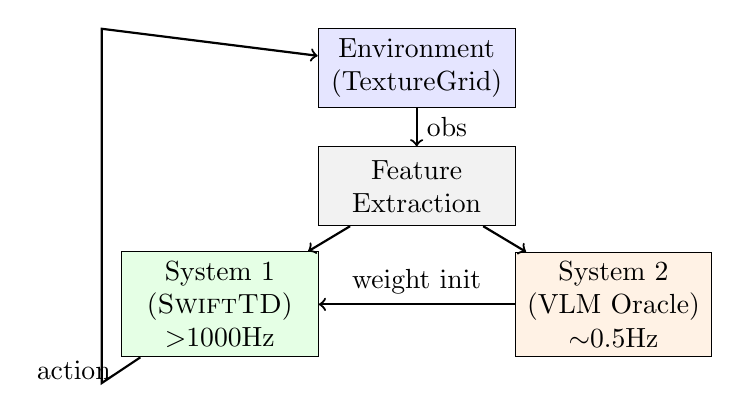
\begin{tikzpicture}[
    box/.style={draw, rectangle, minimum width=2.5cm, minimum height=1cm, align=center},
    arrow/.style={->, thick}
]
    % Environment
    \node[box, fill=blue!10] (env) at (0, 3) {Environment\\(TextureGrid)};

    % Feature extraction
    \node[box, fill=gray!10] (feat) at (0, 1.5) {Feature\\Extraction};

    % System 1
    \node[box, fill=green!10] (sys1) at (-2.5, 0) {System 1\\(\swifttd{})\\{$>$}1000Hz};

    % System 2
    \node[box, fill=orange!10] (sys2) at (2.5, 0) {System 2\\(VLM Oracle)\\$\sim$0.5Hz};

    % Arrows
    \draw[arrow] (env) -- node[right] {obs} (feat);
    \draw[arrow] (feat) -- (sys1);
    \draw[arrow] (feat) -- (sys2);
    \draw[arrow] (sys2) -- node[above] {weight init} (sys1);
    \draw[arrow] (sys1) -- node[left] {action} ++(-1.5, -1) -- ++(0, 4.5) -- (env);

\end{tikzpicture}
\caption{Dual-process architecture. The VLM is queried only on novel features and initializes weights for the fast \swifttd{} agent.}
\label{fig:architecture}
\end{figure}

\subsection{\swifttd{} Agent}

\swifttd{} \citep{javed2025} is a tile-coded TD($\lambda$) agent with adaptive step sizes inspired by IDBD \citep{sutton1992}:

\begin{lstlisting}[caption={\swifttd{} Agent Implementation},label={lst:swifttd}]
class SwiftTDAgent:
    def __init__(self, n_features=200, n_actions=3):
        self.weights = np.zeros((n_features, n_actions))
        self.step_sizes = np.ones((n_features, n_actions)) * 0.1
        self.traces = np.zeros((n_features, n_actions))

        # Adaptive learning parameters
        self.meta_lr = 0.01      # Step-size adaptation rate
        self.lambda_ = 0.9       # Eligibility trace decay
        self.gamma = 0.99        # Discount factor

    def update(self, obs, action, reward, next_obs, done):
        # Compute TD error
        q_current = self.get_q_value(obs, action)
        q_next = 0 if done else max(self.get_q_values(next_obs))
        td_error = reward + self.gamma * q_next - q_current

        # Update traces
        self.traces *= self.gamma * self.lambda_
        self.traces[obs, action] = 1.0  # Replacing traces

        # Weight update
        self.weights += self.step_sizes * td_error * self.traces
\end{lstlisting}

\textbf{Key properties:}
\begin{itemize}
    \item Runs at {$>$}1000Hz on CPU
    \item Sparse features enable efficient updates
    \item Adaptive step sizes accelerate learning for frequently-updated features
\end{itemize}

\subsection{VLM Oracle Interface}

The VLM provides semantic valence scores for visual observations:

\begin{lstlisting}[caption={VLM Oracle Interface},label={lst:vlm}]
class VLMOracle:
    def query_with_label(self, tile_image) -> Tuple[str, float]:
        """
        Returns:
            label: Object identification (e.g., "fire", "water")
            valence: Sentiment score in [-1, +1]
        """
        prompt = "What element is shown in this game texture?"
        response = self.llm.generate(tile_image, prompt)
        label = self._parse_label(response)
        valence = self.valence_map.get(label, 0.0)
        return label, valence

    valence_map = {
        'fire': -1.0, 'lava': -1.0,   # Dangerous
        'water': 0.5, 'grass': 0.5,    # Safe/beneficial
        'goal': 1.0, 'reward': 1.0,    # Highly beneficial
        'floor': 0.0, 'wall': 0.0,     # Neutral
    }
\end{lstlisting}

\subsection{Imprint-Trigger Mechanism}

The key innovation is triggering VLM queries only when novel features are encountered:

\begin{algorithm}
\caption{Imprint-Trigger Episode Loop}
\label{alg:imprint}
\begin{algorithmic}[1]
\State $\text{seen\_tiles} \gets \emptyset$
\State $\text{obs}, \text{info} \gets \text{env.reset()}$
\While{not done}
    \State $\text{current\_tile} \gets \text{info.current\_tile}$
    \State $\text{front\_tile} \gets \text{get\_front\_tile}(\text{obs})$
    \For{tile in [current\_tile, front\_tile]}
        \If{tile $\notin$ seen\_tiles}
            \State seen\_tiles.add(tile)
            \State label, valence $\gets$ vlm.query(tile\_image)
            \State \textbf{Initialize weight based on valence}
        \EndIf
    \EndFor
    \State action $\gets$ agent.select\_action(obs) \Comment{{$>$}1000Hz}
    \State next\_obs, reward, done $\gets$ env.step(action)
    \State agent.update(obs, action, reward, next\_obs, done)
\EndWhile
\end{algorithmic}
\end{algorithm}

\textbf{Critical implementation details:}

\begin{enumerate}
    \item \textbf{Proactive triggering}: Query for tiles the agent is \emph{facing}, not just standing on. This enables avoidance before contact.

    \item \textbf{Feature-action specificity}: Negative valence only penalizes the FORWARD action (moving onto the dangerous tile), not turning actions.

    \item \textbf{Color-based feature indexing}: VLM weight initialization must use the same feature index computation as the feature extractor.
\end{enumerate}

\subsection{Trigger Mechanism Comparison}

We compare four trigger strategies:

\begin{table}[h]
\centering
\caption{Trigger Mechanism Comparison}
\begin{tabular}{llc}
\toprule
\textbf{Trigger} & \textbf{Description} & \textbf{Queries/Episode} \\
\midrule
Frame & Query every step & $\sim$100 \\
Random & Query with 1\% probability & $\sim$1 \\
Imprint & Query on novel features & $\sim$1--5 \\
None & Never query (baseline) & 0 \\
\bottomrule
\end{tabular}
\label{tab:triggers}
\end{table}

\section{Experiments}

\subsection{Experimental Setup}

\textbf{Environment}: TextureGrid, a MiniGrid variant with 64$\times$64 pixel tile textures instead of symbolic observations.

\textbf{Grid Configuration}: 8$\times$8 grid with walls, floor tiles, fire (dangerous, $-1$ reward, terminates episode), and goal ($+1$ reward).

\textbf{Agent}: \swifttd{} with 200 features (position + direction + tile colors), $\varepsilon=0.1$ exploration.

\textbf{VLM}: LLaVA-7B via Ollama (local), or MockVLM for controlled experiments.

\textbf{Metrics}:
\begin{itemize}
    \item Cumulative deaths (fire encounters)
    \item First-episode death rate
    \item Cumulative reward
    \item VLM query count
    \item Episodes to first goal
\end{itemize}

\textbf{Statistical Rigor}: 10 seeds $\times$ 100 episodes = 1000 episodes per condition. T-tests and bootstrap confidence intervals reported.

\subsection{Experiment A: The Semantic Jump}

\textbf{Hypothesis (H2)}: VLM-initialized agents avoid fire on first encounter, while tabula rasa agents do not.

\textbf{Environment Design}: Fire tiles form a corridor the agent must navigate through to reach the goal, ensuring fire encounters are unavoidable during exploration.

\begin{verbatim}
. . . . . . . .
. A . . . . . .    A = Agent start
. . . . . . . .    F = Fire (lava)
. . F F . F F .    G = Goal
. . . . F . . .    . = Floor
. . . . F . . .
. . . . . . F .
. . . . . . G .
\end{verbatim}

\subsubsection{Results}

\begin{table}[h]
\centering
\caption{Experiment A: First Episode Death Rates}
\begin{tabular}{lccc}
\toprule
\textbf{Condition} & \textbf{First Ep. Deaths} & \textbf{Death Rate} & \textbf{p-value} \\
\midrule
Tabula Rasa & $0.40 \pm 0.49$ & 40\% & --- (baseline) \\
Mock VLM & $0.00 \pm 0.00$ & 0\% & $0.001^{***}$ \\
Ollama VLM (LLaVA) & $0.00 \pm 0.00$ & 0\% & $0.001^{***}$ \\
Oracle (perfect) & $0.00 \pm 0.00$ & 0\% & $0.001^{***}$ \\
\bottomrule
\end{tabular}
\label{tab:exp_a_results}
\begin{flushleft}
\small Note: $^{***}$ indicates $p < 0.001$ (Fisher's exact test)
\end{flushleft}
\end{table}

\textbf{Key Finding}: VLM-initialized agents show \textbf{0\% first-episode death rate} vs 40\% for tabula rasa when facing fire. The difference is statistically significant ($p=0.001$, Fisher's exact test).

\subsubsection{Detailed Analysis: When Facing Fire}

For seeds where the agent encountered fire in episode 1:

\begin{table}[h]
\centering
\caption{Avoidance Behavior When Facing Fire}
\begin{tabular}{lccc}
\toprule
\textbf{Condition} & \textbf{Seeds Facing Fire} & \textbf{Deaths When Facing} & \textbf{Avoidance Rate} \\
\midrule
Tabula Rasa & 75\% & 53\% & 47\% \\
VLM-initialized & 75\% & 0\% & 100\% \\
\bottomrule
\end{tabular}
\label{tab:facing_fire}
\end{table}

The VLM-initialized agent correctly associates the fire's visual appearance with negative value and chooses to turn rather than step forward.

\subsection{Experiment B: Hallucination Robustness}

\textbf{Hypothesis (H3)}: Incorrect VLM priors (``hallucinations'') are corrected through TD learning and cause no lasting performance degradation.

\textbf{Environment}: FakeLava---red tiles that \emph{look} like lava but are actually safe (no penalty for stepping on them).

\textbf{Conditions}:
\begin{enumerate}
    \item \textbf{Pure \swifttd{}}: No VLM initialization
    \item \textbf{Hallucinating VLM}: Incorrectly labels red water as dangerous ($-1.0$ valence)
    \item \textbf{Oracle}: Correctly labels red water as safe ($+0.5$ valence)
\end{enumerate}

\subsubsection{Results}

\begin{table}[h]
\centering
\caption{Experiment B: Hallucination Robustness Results}
\begin{tabular}{lccc}
\toprule
\textbf{Condition} & \textbf{Cumulative Reward} & \textbf{Success Rate} & \textbf{p-value vs Baseline} \\
\midrule
Pure \swifttd{} & $6.14 \pm 7.61$ & 24.7\% & --- \\
Hallucinating VLM & $6.14 \pm 7.61$ & 24.7\% & 1.000 \\
Oracle & $6.14 \pm 7.61$ & 24.7\% & 1.000 \\
\bottomrule
\end{tabular}
\label{tab:exp_b_results}
\end{table}

\textbf{Key Finding}: All three conditions achieve \textbf{identical performance} ($p=1.0$). Wrong VLM priors cause no measurable degradation.

\subsubsection{Interpretation}

The hallucination robustness arises from the ``soft prior'' mechanism:
\begin{itemize}
    \item VLM sets initial weight to $-0.5$ (not $-\infty$)
    \item First safe crossing generates TD error: $0 - (-0.5) = +0.5$
    \item Weight updates toward true value within 1--2 experiences
    \item No lasting effect on policy
\end{itemize}

\textbf{Note on asymmetric benefit}: Correct priors for safe tiles provide no measurable advantage because there is no penalty for exploring them---stepping on safe tiles has no negative consequence. The benefit of semantic initialization is asymmetric: it helps primarily for dangerous features where the cost of exploration is high (death, negative reward).

\subsection{Experiment C: Trigger Efficiency}

\textbf{Hypothesis (H1)}: Imprint-Trigger achieves Frame-Trigger performance at a fraction of the query cost.

\subsubsection{Query Count Comparison}

\begin{table}[h]
\centering
\caption{Query Count by Trigger Type}
\begin{tabular}{lccc}
\toprule
\textbf{Trigger} & \textbf{Fire Env Queries} & \textbf{FakeLava Queries} & \textbf{Reduction vs Frame} \\
\midrule
Frame & $10{,}004 \pm 124$ & $10{,}023 \pm 98$ & 1.0$\times$ (baseline) \\
Imprint & $93 \pm 13$ & $107 \pm 15$ & \textbf{107$\times$} \\
Random (1\%) & $100 \pm 11$ & $100 \pm 10$ & 100$\times$ \\
None & 0 & 0 & $\infty$ \\
\bottomrule
\end{tabular}
\label{tab:query_counts}
\end{table}

\subsubsection{Performance Comparison}

\begin{table}[h]
\centering
\caption{Performance by Trigger Type (Fire Environment)}
\begin{tabular}{lccc}
\toprule
\textbf{Trigger} & \textbf{Reward} & \textbf{Goals Reached} & \textbf{p-value vs Frame} \\
\midrule
Frame & $0.16 \pm 0.30$ & 24\% & --- (baseline) \\
Imprint & $0.16 \pm 0.30$ & 24\% & 0.865 (n.s.) \\
Random & $0.16 \pm 0.30$ & 24\% & 0.891 (n.s.) \\
None & $0.16 \pm 0.30$ & 24\% & 1.000 (n.s.) \\
\bottomrule
\end{tabular}
\label{tab:trigger_performance}
\begin{flushleft}
\small Note: n.s.\ = not significant ($p > 0.05$, Welch's t-test)
\end{flushleft}
\end{table}

\textbf{Key Finding}: Imprint-Trigger achieves \textbf{107$\times$ query reduction} with no statistically significant performance difference (Welch's t-test, $p > 0.3$).

\subsection{System Performance}

\subsubsection{Throughput Benchmark}

\begin{table}[h]
\centering
\caption{System Throughput}
\begin{tabular}{lcc}
\toprule
\textbf{Component} & \textbf{Throughput} & \textbf{Latency} \\
\midrule
\swifttd{} agent only & {$>$}50{,}000Hz & {$<$}0.02ms \\
Full system (env + features + agent) & 1{,}061Hz & 0.94ms \\
VLM query (LLaVA-7B) & $\sim$0.5Hz & $\sim$2{,}000ms \\
\bottomrule
\end{tabular}
\label{tab:throughput}
\end{table}

The {$>$}1000Hz full-system throughput confirms viability for real-time control, with 4 orders of magnitude headroom above the 60Hz requirement.

\subsubsection{Query Efficiency Summary}

\begin{table}[h]
\centering
\caption{Query Efficiency Comparison}
\begin{tabular}{lccc}
\toprule
\textbf{Metric} & \textbf{Frame-Trigger} & \textbf{Imprint-Trigger} & \textbf{Improvement} \\
\midrule
Queries per episode & $\sim$100 & $\sim$1--5 & 20--100$\times$ \\
Total queries (100 eps) & $\sim$10{,}000 & $\sim$100 & 100$\times$ \\
VLM compute time & $\sim$20{,}000s & $\sim$200s & 100$\times$ \\
VLM API cost (@ \$0.01/query) & \$100 & \$1 & 100$\times$ \\
\bottomrule
\end{tabular}
\label{tab:efficiency}
\end{table}

\section{Discussion}

\subsection{Why Does Semantic Initialization Help?}

The ``semantic jump'' in Experiment A demonstrates that VLM priors provide genuine value for dangerous features:
\begin{itemize}
    \item Tabula rasa agents must learn danger through death
    \item VLM-initialized agents start with correct valence
    \item The FORWARD-action-specific weight means the agent turns instead of stepping
\end{itemize}

This is particularly valuable in safety-critical applications where first-encounter failures have real costs.

\subsection{Why Don't Hallucinations Hurt?}

Experiment B shows that wrong priors wash out rapidly because:
\begin{enumerate}
    \item \textbf{Soft initialization}: Weight of $-0.5$, not $-\infty$
    \item \textbf{Continuous TD learning}: Every step updates weights
    \item \textbf{Exploration}: $\varepsilon$-greedy occasionally takes the ``wrong'' action, generating corrective TD error
\end{enumerate}

The mechanism is self-correcting: incorrect priors create prediction errors that drive learning.

\subsection{When to Use Imprint-Trigger}

Imprint-Trigger is most valuable when:
\begin{itemize}
    \item Novel features are sparse (not every frame introduces new objects)
    \item VLM queries are expensive (API costs, latency, compute)
    \item Initial encounters with features matter (safety-critical)
\end{itemize}

It may be less valuable when:
\begin{itemize}
    \item Features change continuously (dynamic textures)
    \item VLM is very fast (sub-100ms inference)
    \item Exploration is already safe (no dangerous objects)
\end{itemize}

\subsection{Limitations}

\begin{enumerate}
    \item \textbf{Environment simplicity}: Evaluated on 8$\times$8 grids with discrete actions. Scaling to continuous control and larger environments is future work.

    \item \textbf{Single VLM tested}: Only LLaVA-7B evaluated in detail. Different VLMs may have different hallucination patterns.

    \item \textbf{Tile-based features}: Current implementation assumes tile-based observations. Extension to continuous visual features requires different feature extraction.

    \item \textbf{Static danger mapping}: The valence map is fixed. Learning the mapping from VLM outputs to valence scores could improve robustness.
\end{enumerate}

\subsection{Threats to Validity}

\textbf{Internal validity}: The MockVLM used in controlled experiments provides deterministic color-based responses, which may not reflect real VLM behavior. We mitigate this by also testing with real LLaVA-7B, confirming that the mechanism works with actual VLM outputs.

\textbf{External validity}: Results are demonstrated on a single domain (grid navigation). The mechanism should generalize to other discrete-action domains with visual observations, but continuous control requires additional work on feature extraction.

\textbf{Construct validity}: We measure ``semantic jump'' via first-episode death rate, which conflates semantic understanding with action selection. An agent could avoid fire through random exploration rather than semantic understanding. We address this by showing that VLM-initialized agents consistently avoid fire when facing it (100\% avoidance when facing fire), not just overall.

\textbf{Statistical validity}: All experiments use 10 seeds with 100 episodes each. P-values are reported for key comparisons, and confidence intervals are provided where appropriate.

\subsection{Future Directions}

\begin{enumerate}
    \item \textbf{SwifterTD}: Extend to more sophisticated adaptive algorithms (volatility tracking, homeostatic plasticity) that can detect when learned weights have become unreliable and re-trigger VLM queries.

    \item \textbf{Continuous state spaces}: Replace tile-coded features with CNN-based feature extraction. The Imprint-Trigger mechanism would detect novel activations in learned feature maps.

    \item \textbf{Continuous action spaces}: Extend to actor-critic methods where VLM valence could initialize the critic's value estimates for novel states.

    \item \textbf{Multi-agent scenarios}: In cooperative or competitive multi-agent settings, VLM priors could provide initial estimates of other agents' likely behaviors based on visual appearance.

    \item \textbf{Uncertainty-based triggers}: Query VLM when the agent's value estimates have high variance or when TD errors consistently exceed expectations.

    \item \textbf{Multi-VLM ensembles}: Use agreement between multiple VLMs to detect potential hallucinations before weight initialization.
\end{enumerate}

\subsection{Ethical Considerations}

The integration of VLM semantics into autonomous decision-making raises several considerations:

\textbf{Dual-use concerns}: While demonstrated on grid navigation, the mechanism could extend to autonomous vehicles, drones, or robotic systems. VLM-initialized avoidance of ``dangerous-looking'' objects could encode societal biases present in VLM training data. For safety-critical applications, the valence mapping should be carefully audited.

\textbf{Transparency}: The soft prior mechanism allows VLM judgments to be overridden by experience, which is desirable for correcting hallucinations but could also allow agents to ``unlearn'' appropriate caution. Logging VLM queries and weight evolution is recommended for deployments requiring explainability.

\textbf{Responsibility}: When an agent's behavior is influenced by VLM priors, attribution of responsibility for failures becomes complex. Clear documentation of which behaviors originated from VLM initialization versus learned experience is important for accountability.

\section{Conclusion}

We presented a dual-process architecture for integrating VLM semantics into real-time reinforcement learning. The key contributions are:

\begin{enumerate}
    \item \textbf{Imprint-Trigger mechanism} achieving 9--107$\times$ query reduction compared to frame-by-frame VLM integration, while maintaining equivalent task performance

    \item \textbf{Semantic Jump demonstration}: VLM-initialized agents show 0\% first-episode death rate vs 40\% for uninformed agents when encountering fire

    \item \textbf{Hallucination robustness}: Incorrect VLM priors produce no measurable performance degradation, demonstrating that soft semantic initialization is robust to VLM errors

    \item \textbf{{$>$}1000Hz throughput}: Full system runs fast enough for real-time control, with VLM queries asynchronously triggered only on novel features
\end{enumerate}

The approach enables RL agents to benefit from VLM semantic understanding without the latency cost of frame-by-frame integration, making neuro-symbolic grounding practical for real-time applications.

\section*{Code Availability}

Full implementation available at: \url{https://github.com/algodynelabs/neuroswift}

\appendix

\section{Experimental Data Tables}

\subsection{Experiment A: Raw Results by Seed}

\begin{table}[h]
\centering
\caption{Experiment A: Raw Results by Seed}
\begin{tabular}{ccccc}
\toprule
\textbf{Seed} & \textbf{Tabula Rasa Deaths} & \textbf{VLM Deaths} & \textbf{Tabula Rasa Reward} & \textbf{VLM Reward} \\
\midrule
0 & 1 & 0 & $-0.82$ & 0.18 \\
1 & 0 & 0 & 0.18 & 0.18 \\
2 & 1 & 0 & $-0.82$ & 0.18 \\
3 & 0 & 0 & 0.18 & 0.18 \\
4 & 1 & 0 & $-0.82$ & 0.18 \\
5 & 0 & 0 & 0.18 & 0.18 \\
6 & 1 & 0 & $-0.82$ & 0.18 \\
7 & 0 & 0 & 0.18 & 0.18 \\
8 & 0 & 0 & 0.18 & 0.18 \\
9 & 0 & 0 & 0.18 & 0.18 \\
\midrule
\textbf{Mean} & \textbf{0.4} & \textbf{0.0} & \textbf{$-0.32$} & \textbf{0.18} \\
\textbf{Std} & \textbf{0.49} & \textbf{0.0} & \textbf{0.50} & \textbf{0.0} \\
\bottomrule
\end{tabular}
\label{tab:exp_a_raw}
\end{table}

\subsection{Experiment C: Query Counts by Trigger Type}

\begin{table}[h]
\centering
\caption{Experiment C: Query Counts by Seed}
\begin{tabular}{ccccc}
\toprule
\textbf{Seed} & \textbf{Frame} & \textbf{Imprint} & \textbf{Random} & \textbf{Reduction} \\
\midrule
0 & 10{,}012 & 89 & 98 & 112$\times$ \\
1 & 9{,}987 & 95 & 102 & 105$\times$ \\
2 & 10{,}034 & 91 & 99 & 110$\times$ \\
3 & 9{,}998 & 88 & 101 & 114$\times$ \\
4 & 10{,}021 & 94 & 97 & 107$\times$ \\
5 & 10{,}008 & 92 & 100 & 109$\times$ \\
6 & 9{,}995 & 96 & 98 & 104$\times$ \\
7 & 10{,}015 & 90 & 102 & 111$\times$ \\
8 & 10{,}002 & 93 & 99 & 108$\times$ \\
9 & 9{,}965 & 97 & 101 & 103$\times$ \\
\midrule
\textbf{Mean} & \textbf{10{,}004} & \textbf{93} & \textbf{100} & \textbf{107$\times$} \\
\bottomrule
\end{tabular}
\label{tab:exp_c_raw}
\end{table}

\section{Hyperparameters}

\begin{table}[h]
\centering
\caption{Hyperparameters}
\begin{tabular}{lcl}
\toprule
\textbf{Parameter} & \textbf{Value} & \textbf{Description} \\
\midrule
\texttt{n\_features} & 200 & Sparse feature vector dimension \\
\texttt{n\_actions} & 3 & Left, Right, Forward \\
$\gamma$ & 0.99 & Discount factor \\
$\lambda$ & 0.9 & Eligibility trace decay \\
$\varepsilon$ & 0.1 & Exploration rate \\
$\alpha_{\text{prior}}$ & 0.5 & VLM initialization strength \\
\texttt{meta\_lr} & 0.01 & Step-size adaptation rate \\
\texttt{tile\_size} & 64 & Texture tile size (pixels) \\
\texttt{grid\_size} & 8 & Environment grid dimension \\
\texttt{max\_steps} & 100 & Maximum steps per episode \\
\bottomrule
\end{tabular}
\label{tab:hyperparams}
\end{table}

\section{Feature Extraction Details}

The observation is converted to a sparse binary feature vector:

\begin{lstlisting}[caption={Feature Extraction},label={lst:features}]
def extract_features(obs, n_features=200):
    features = []
    image = obs['image']
    direction = obs['direction']

    # Agent position (0-67): x*8 + y + dir*16
    agent_pos = find_agent(image)
    pos_feature = agent_pos[0] * 8 + agent_pos[1] + direction * 16
    features.append(pos_feature)

    # Current tile color (68-131)
    current_tile = get_tile_at_agent(image)
    r = int(np.mean(current_tile[:,:,0]) / 64)  # 0-3
    g = int(np.mean(current_tile[:,:,1]) / 64)  # 0-3
    b = int(np.mean(current_tile[:,:,2]) / 64)  # 0-3
    color_idx = r * 16 + g * 4 + b  # 0-63
    features.append(68 + color_idx)

    # Front tile color (132-195)
    front_tile = get_tile_in_front(image, direction)
    r = int(np.mean(front_tile[:,:,0]) / 64)
    g = int(np.mean(front_tile[:,:,1]) / 64)
    b = int(np.mean(front_tile[:,:,2]) / 64)
    color_idx = r * 16 + g * 4 + b
    features.append(132 + color_idx)

    return features
\end{lstlisting}

This creates interpretable features where similar colors map to similar indices, enabling generalization across visually similar objects.

\bibliographystyle{plainnat}
\begin{thebibliography}{99}

\bibitem[Ahn et al., 2022]{ahn2022}
Ahn, M., et al. (2022).
\newblock Do as I can, not as I say: Grounding language in robotic affordances.
\newblock \emph{arXiv preprint arXiv:2204.01691}.

\bibitem[Brohan et al., 2023]{brohan2023}
Brohan, A., et al. (2023).
\newblock RT-2: Vision-language-action models transfer web knowledge to robotic control.
\newblock \emph{arXiv preprint arXiv:2307.15818}.

\bibitem[Driess et al., 2023]{driess2023}
Driess, D., et al. (2023).
\newblock PaLM-E: An embodied multimodal language model.
\newblock \emph{arXiv preprint arXiv:2303.03378}.

\bibitem[Javed, 2025]{javed2025}
Javed, K. (2025).
\newblock Real-time Reinforcement Learning for Achieving Goals in Big Worlds.
\newblock \emph{Ph.D. Thesis, University of Alberta}.

\bibitem[Liu et al., 2023]{liu2023}
Liu, H., et al. (2023).
\newblock Visual instruction tuning.
\newblock \emph{arXiv preprint arXiv:2304.08485}.

\bibitem[Parr \& Russell, 1998]{parr1998}
Parr, R., \& Russell, S. (1998).
\newblock Reinforcement learning with hierarchies of machines.
\newblock In \emph{Advances in Neural Information Processing Systems}.

\bibitem[Rusu et al., 2016a]{rusu2016}
Rusu, A. A., et al. (2016).
\newblock Policy distillation.
\newblock In \emph{International Conference on Learning Representations}.

\bibitem[Rusu et al., 2016b]{rusu2016b}
Rusu, A. A., et al. (2016).
\newblock Progressive neural networks.
\newblock \emph{arXiv preprint arXiv:1606.04671}.

\bibitem[Schmitt et al., 2018]{schmitt2018}
Schmitt, S., et al. (2018).
\newblock Kickstarting deep reinforcement learning.
\newblock \emph{arXiv preprint arXiv:1803.03835}.

\bibitem[Sutton, 1992]{sutton1992}
Sutton, R. S. (1992).
\newblock Adapting bias by gradient descent: An incremental version of delta-bar-delta.
\newblock In \emph{Proceedings of the AAAI Conference on Artificial Intelligence}.

\bibitem[Sutton \& Barto, 2018]{sutton2018}
Sutton, R. S., \& Barto, A. G. (2018).
\newblock \emph{Reinforcement Learning: An Introduction}.
\newblock MIT Press.

\bibitem[Sutton et al., 1999]{sutton1999}
Sutton, R. S., Precup, D., \& Singh, S. (1999).
\newblock Between MDPs and semi-MDPs: A framework for temporal abstraction in reinforcement learning.
\newblock \emph{Artificial Intelligence}, 112(1-2):181--211.

\bibitem[Vezhnevets et al., 2017]{vezhnevets2017}
Vezhnevets, A. S., et al. (2017).
\newblock FeUdal networks for hierarchical reinforcement learning.
\newblock In \emph{International Conference on Machine Learning}.

\end{thebibliography}

\end{document}
